\documentclass{beamer}

\usepackage{pifont}
\usepackage{tikz}
\usetikzlibrary{arrows.meta,positioning, calc}
\usepackage{caption}

\newcommand{\ideaicon}{\ding{72}}
\newcommand{\screenicon}{\ding{229}}
\newcommand{\personicon}{\ding{110}}
\newcommand{\checkicon}{\ding{51}}
\newcommand{\warnicon}{\ding{115}}

\usetheme{metropolis}
\title{Dat-O-Kart}
\date{}
\author{Adaktylos Leonidas Odysseas, Baumgartner Vincent Vitez,\\ Neda Nikkhousarighiyeh, Alexander Grath}
%\institute{Centre for Modern Beamer Themes} % brauchen wir glaub ich nicht
\begin{document}
  \maketitle
  \section{Einführung}
  %
  \begin{frame}{Einführung}
    \begin{itemize}
      \item Kontext
      \item Führung der App
      \item Usability Evaluierung, Weiterentwicklung, und Abschlussbericht
        \begin{itemize}
          \item Nutzertests
          \item Verbesserungen
          \item Schlussfolgerungen
        \end{itemize}
    \end{itemize}
  \end{frame}
  %
  \begin{frame}{Kontext}
    Thema: Offene Daten erlebbar machen

    Prototyp wurde durch Beliebtheit gewählt.
  \end{frame}
    \begin{frame}{Kontext}
    \begin{center}
        Prototyp: "Karte"
        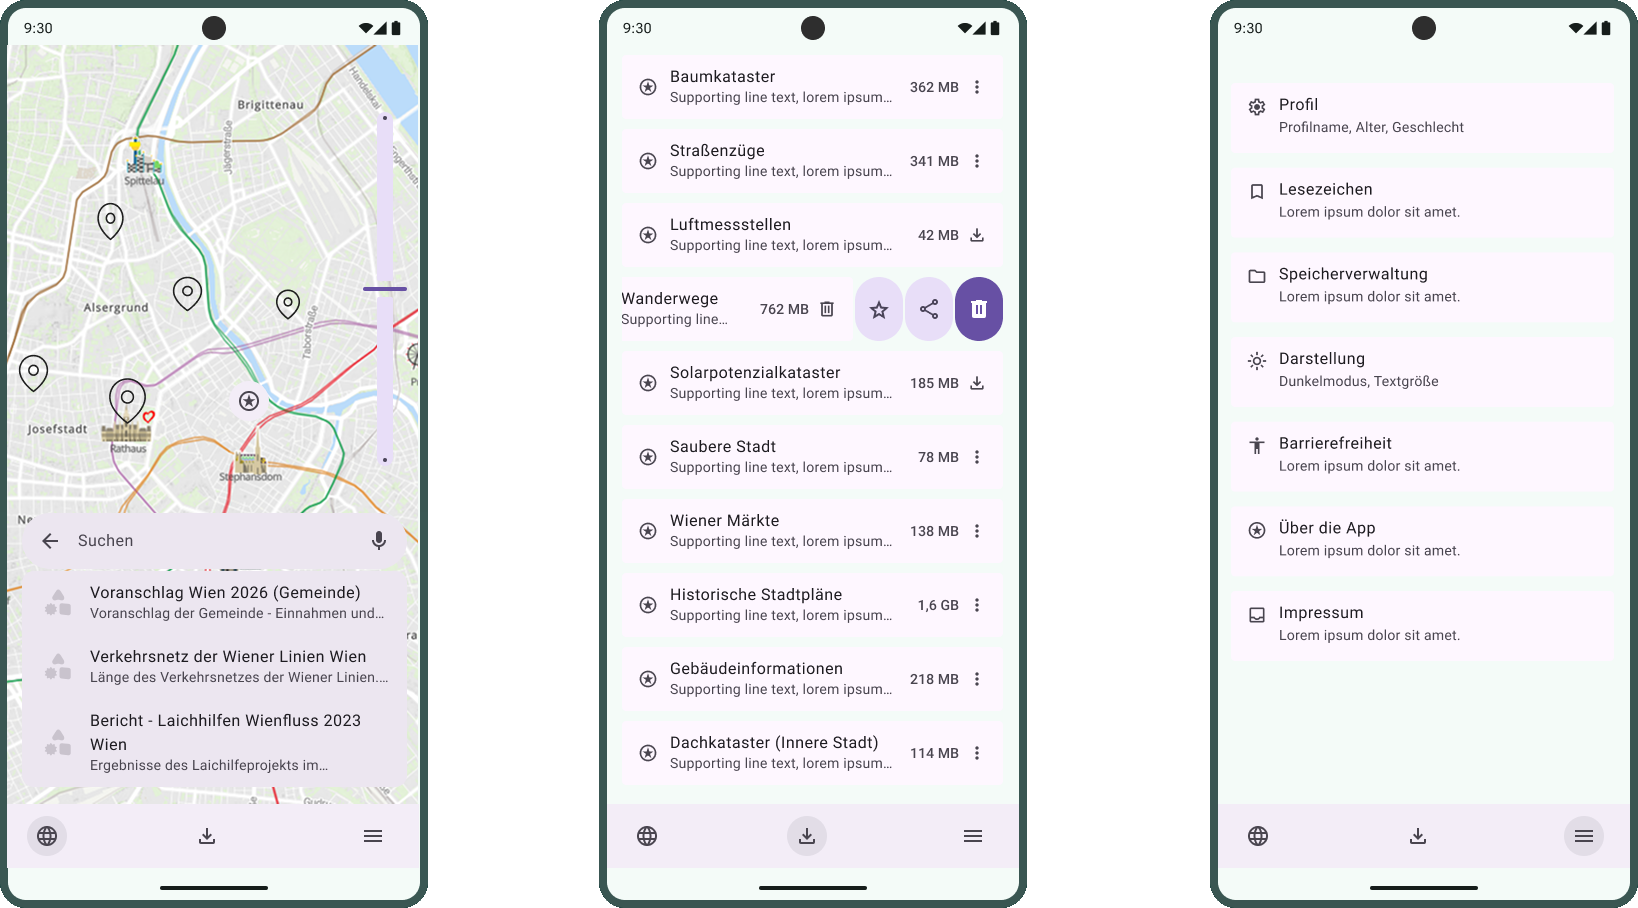
\includegraphics[width=\textwidth]{images/prototype_leonidas.png}
    \end{center}
  \end{frame}
  %
  \begin{frame}{Führung der App}
    Sehen ist verstehen

    Tour der Funktionen
  \end{frame}
  %
  \begin{frame}{Implementation}
    Android Studio Panda 4

    Zielgerät: Pixel 9

    Kotlin und Jetpack Compose

    MapLibre
  \end{frame}
  %
  \begin{frame}{KI Nutzung}
    Gemini eingebunden

    Fast, Ask Modus

    Kontrolle und Validierung
  \end{frame}
  %
  \begin{frame}{Design}
    Material 3

    Modernes Design

    Barrierefrei

    an bekannte Apps angelehnt
  \end{frame}
  %
  \begin{frame}{Lösungsvorschläge}
    Swipen im Downloadtab

    Problem: verstecktes Feature

    Lösung: automatische Anzeige
  \end{frame}
  \begin{frame}{Lösungsvorschläge}
    Unklare Benennung

    \emph{Entdecken} wird zu \emph{Verfügbar} umbenannt
  \end{frame}
    \begin{frame}{Lösungsvorschläge}
    Pin-Überlagerung

    non-issue
  \end{frame}
    \begin{frame}{Lösungsvorschläge}
    Filteroptionen

    für die Zukunft
  \end{frame}
    \begin{frame}{Lösungsvorschläge}
    Hervorheben der Pins

    Pins verdoppeln ihre Größe
  \end{frame}
    \begin{frame}{Lösungsvorschläge}
    Suchvorschläge
  \end{frame}
    \begin{frame}{Ende}
    Vielen Dank für eure Aufmerksamkeit!
  \end{frame}
\end{document}
